\chapter{Beispiele}
\label{cha:Beispiele}
\addtocontents{toc}{\protect\setcounter{tocdepth}{0}}
In diesem Kapitel wollen wir uns die in Kapitel \ref{cha:binomialmodell} und \ref{cha:black-Scholes-Modell} hergeleiteten Algorithmen und Verfahren anschauen. Dazu werden wir zunächst anhand ausgewählter Beispiele die Unterschiede im Konvergenzverhalten für verschiedene Eingabeparameter anschauen.

%%%%%%%%% BINOMIAL BEISPIELE %%%%%%%%%%%%%%%%%%%%%%%%%%%%%%%%%
\section{Binomialmodell}\label{BSP:BINModell}
Im Folgenden werden wir uns die Konvergenz zweier Europäischer Call-Optionen für $K=18$ und $K=20$ zu sonst gleichen Parametern anschauen.
\begin{figure}[h]
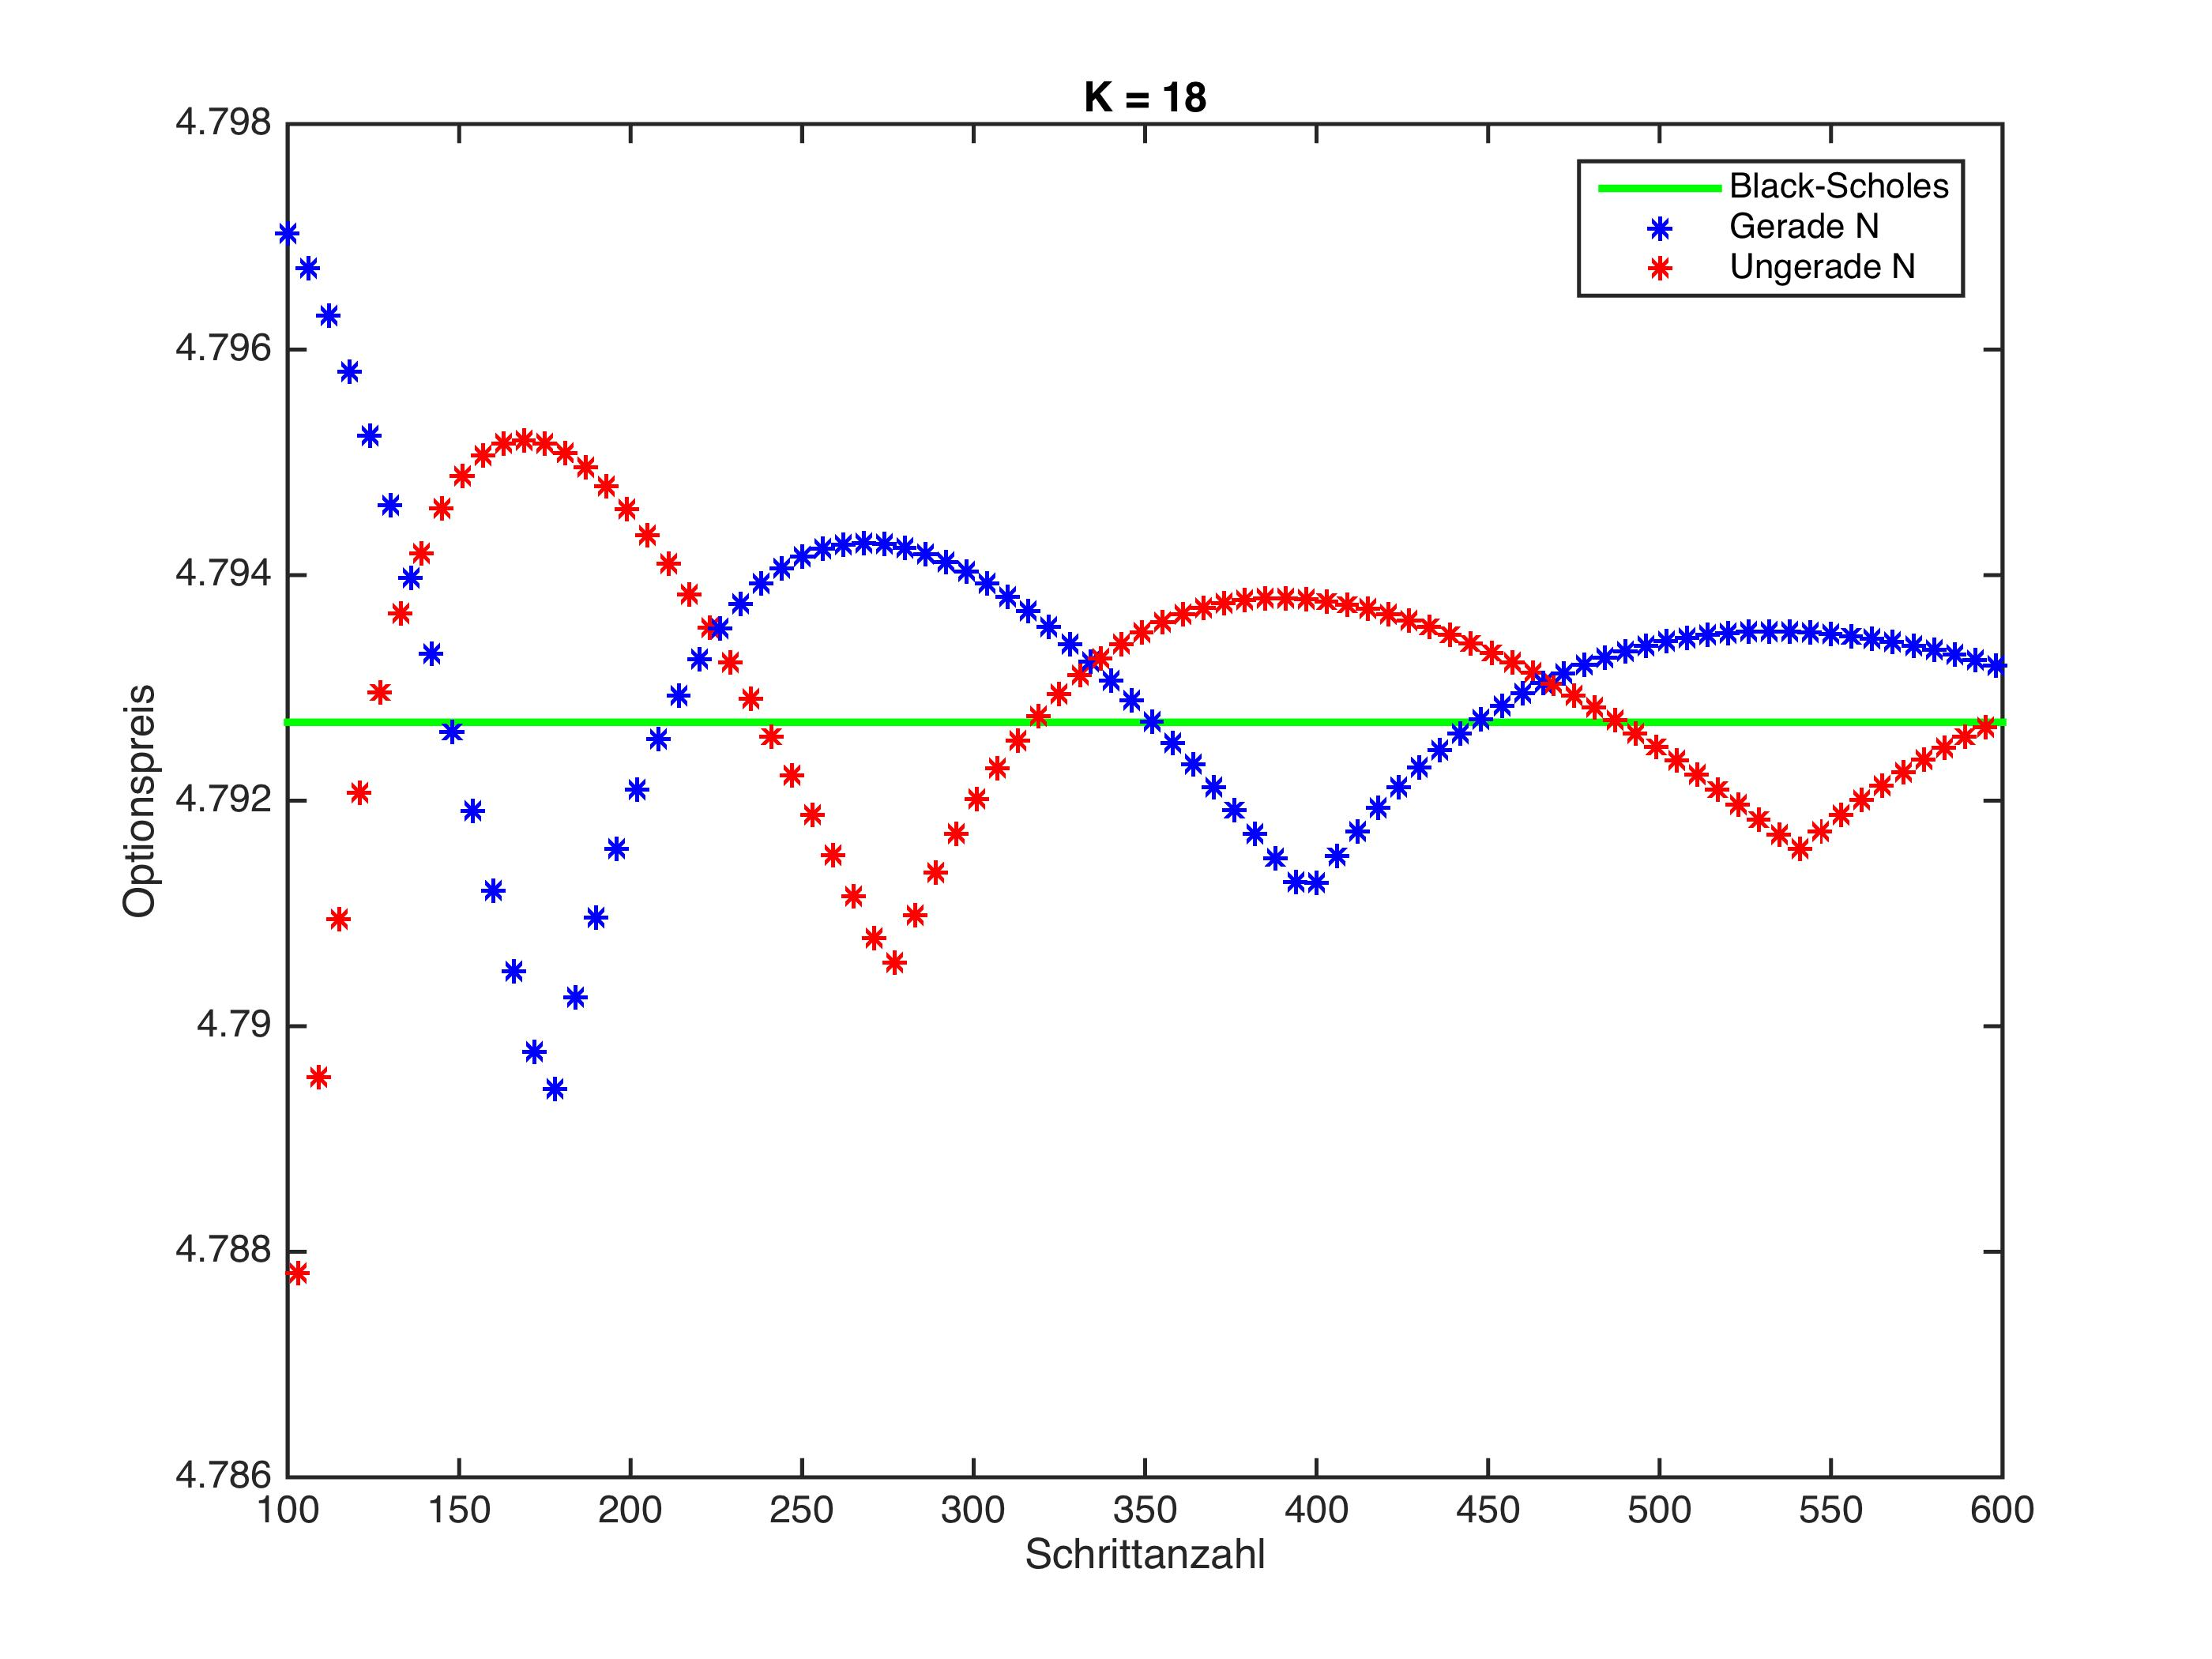
\includegraphics[width=0.45\textwidth]{KonvergenzCall18.jpg}
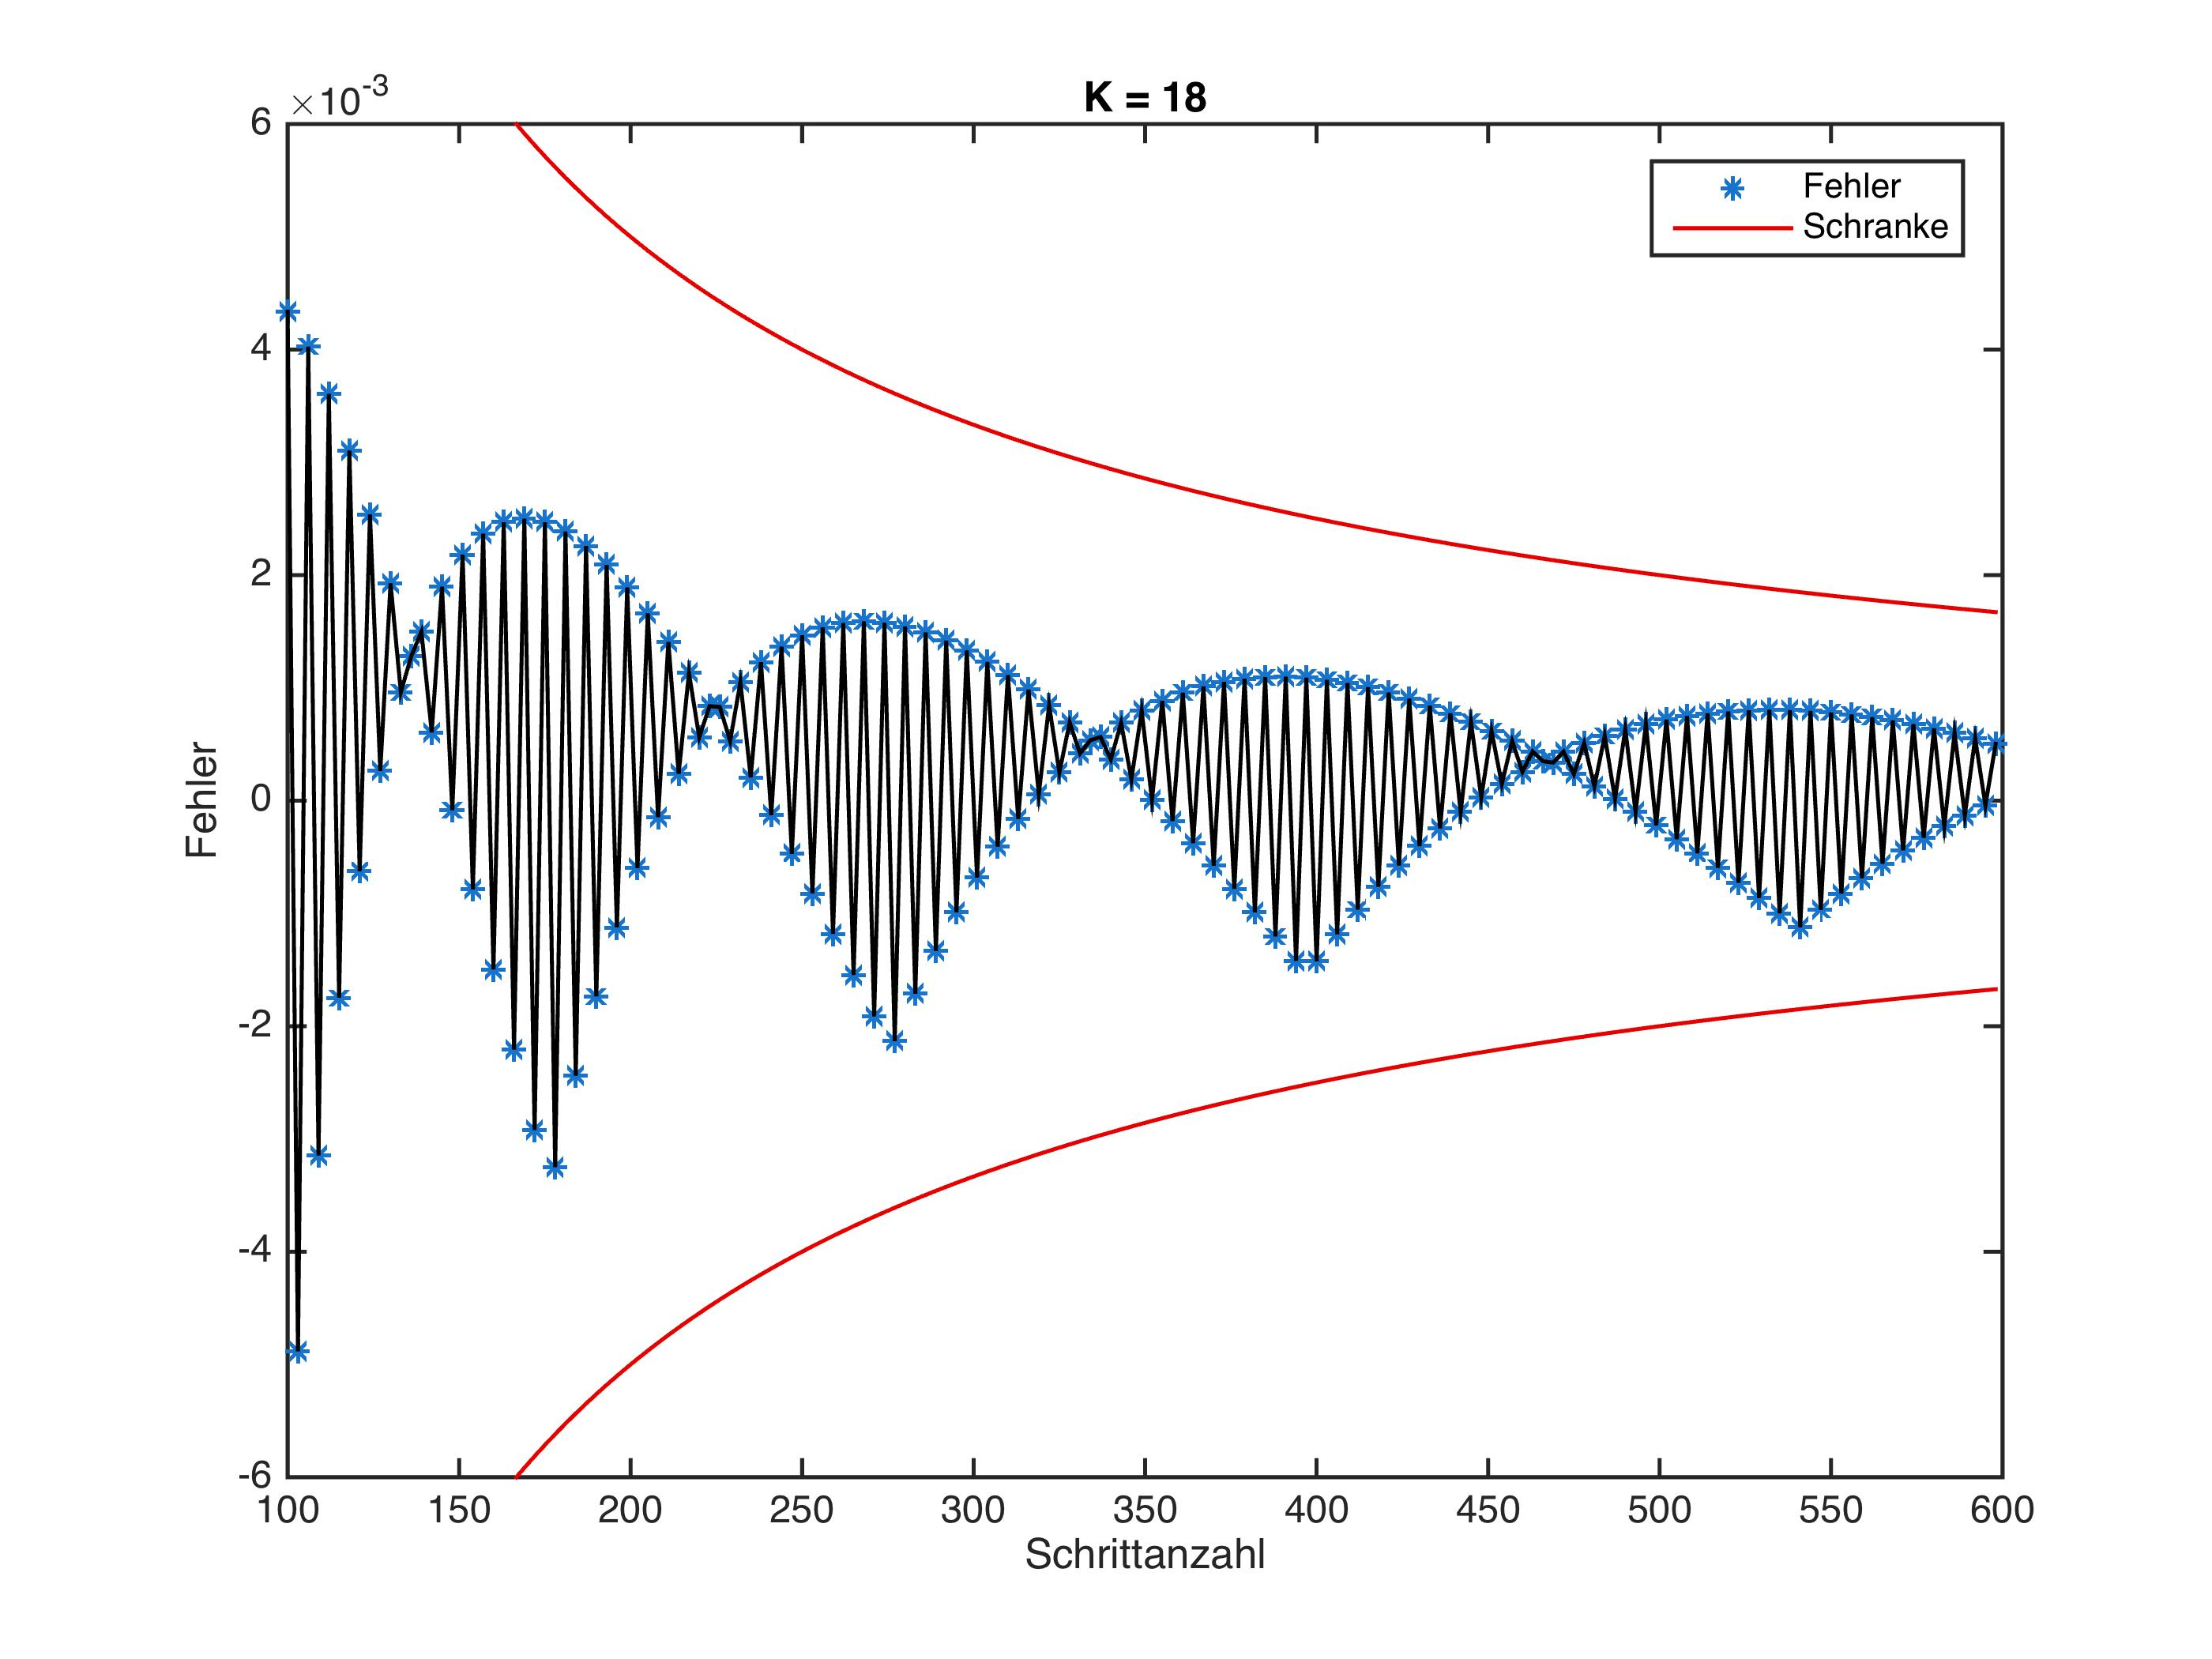
\includegraphics[width=0.45\textwidth]{FehlerCall18.jpg} \\
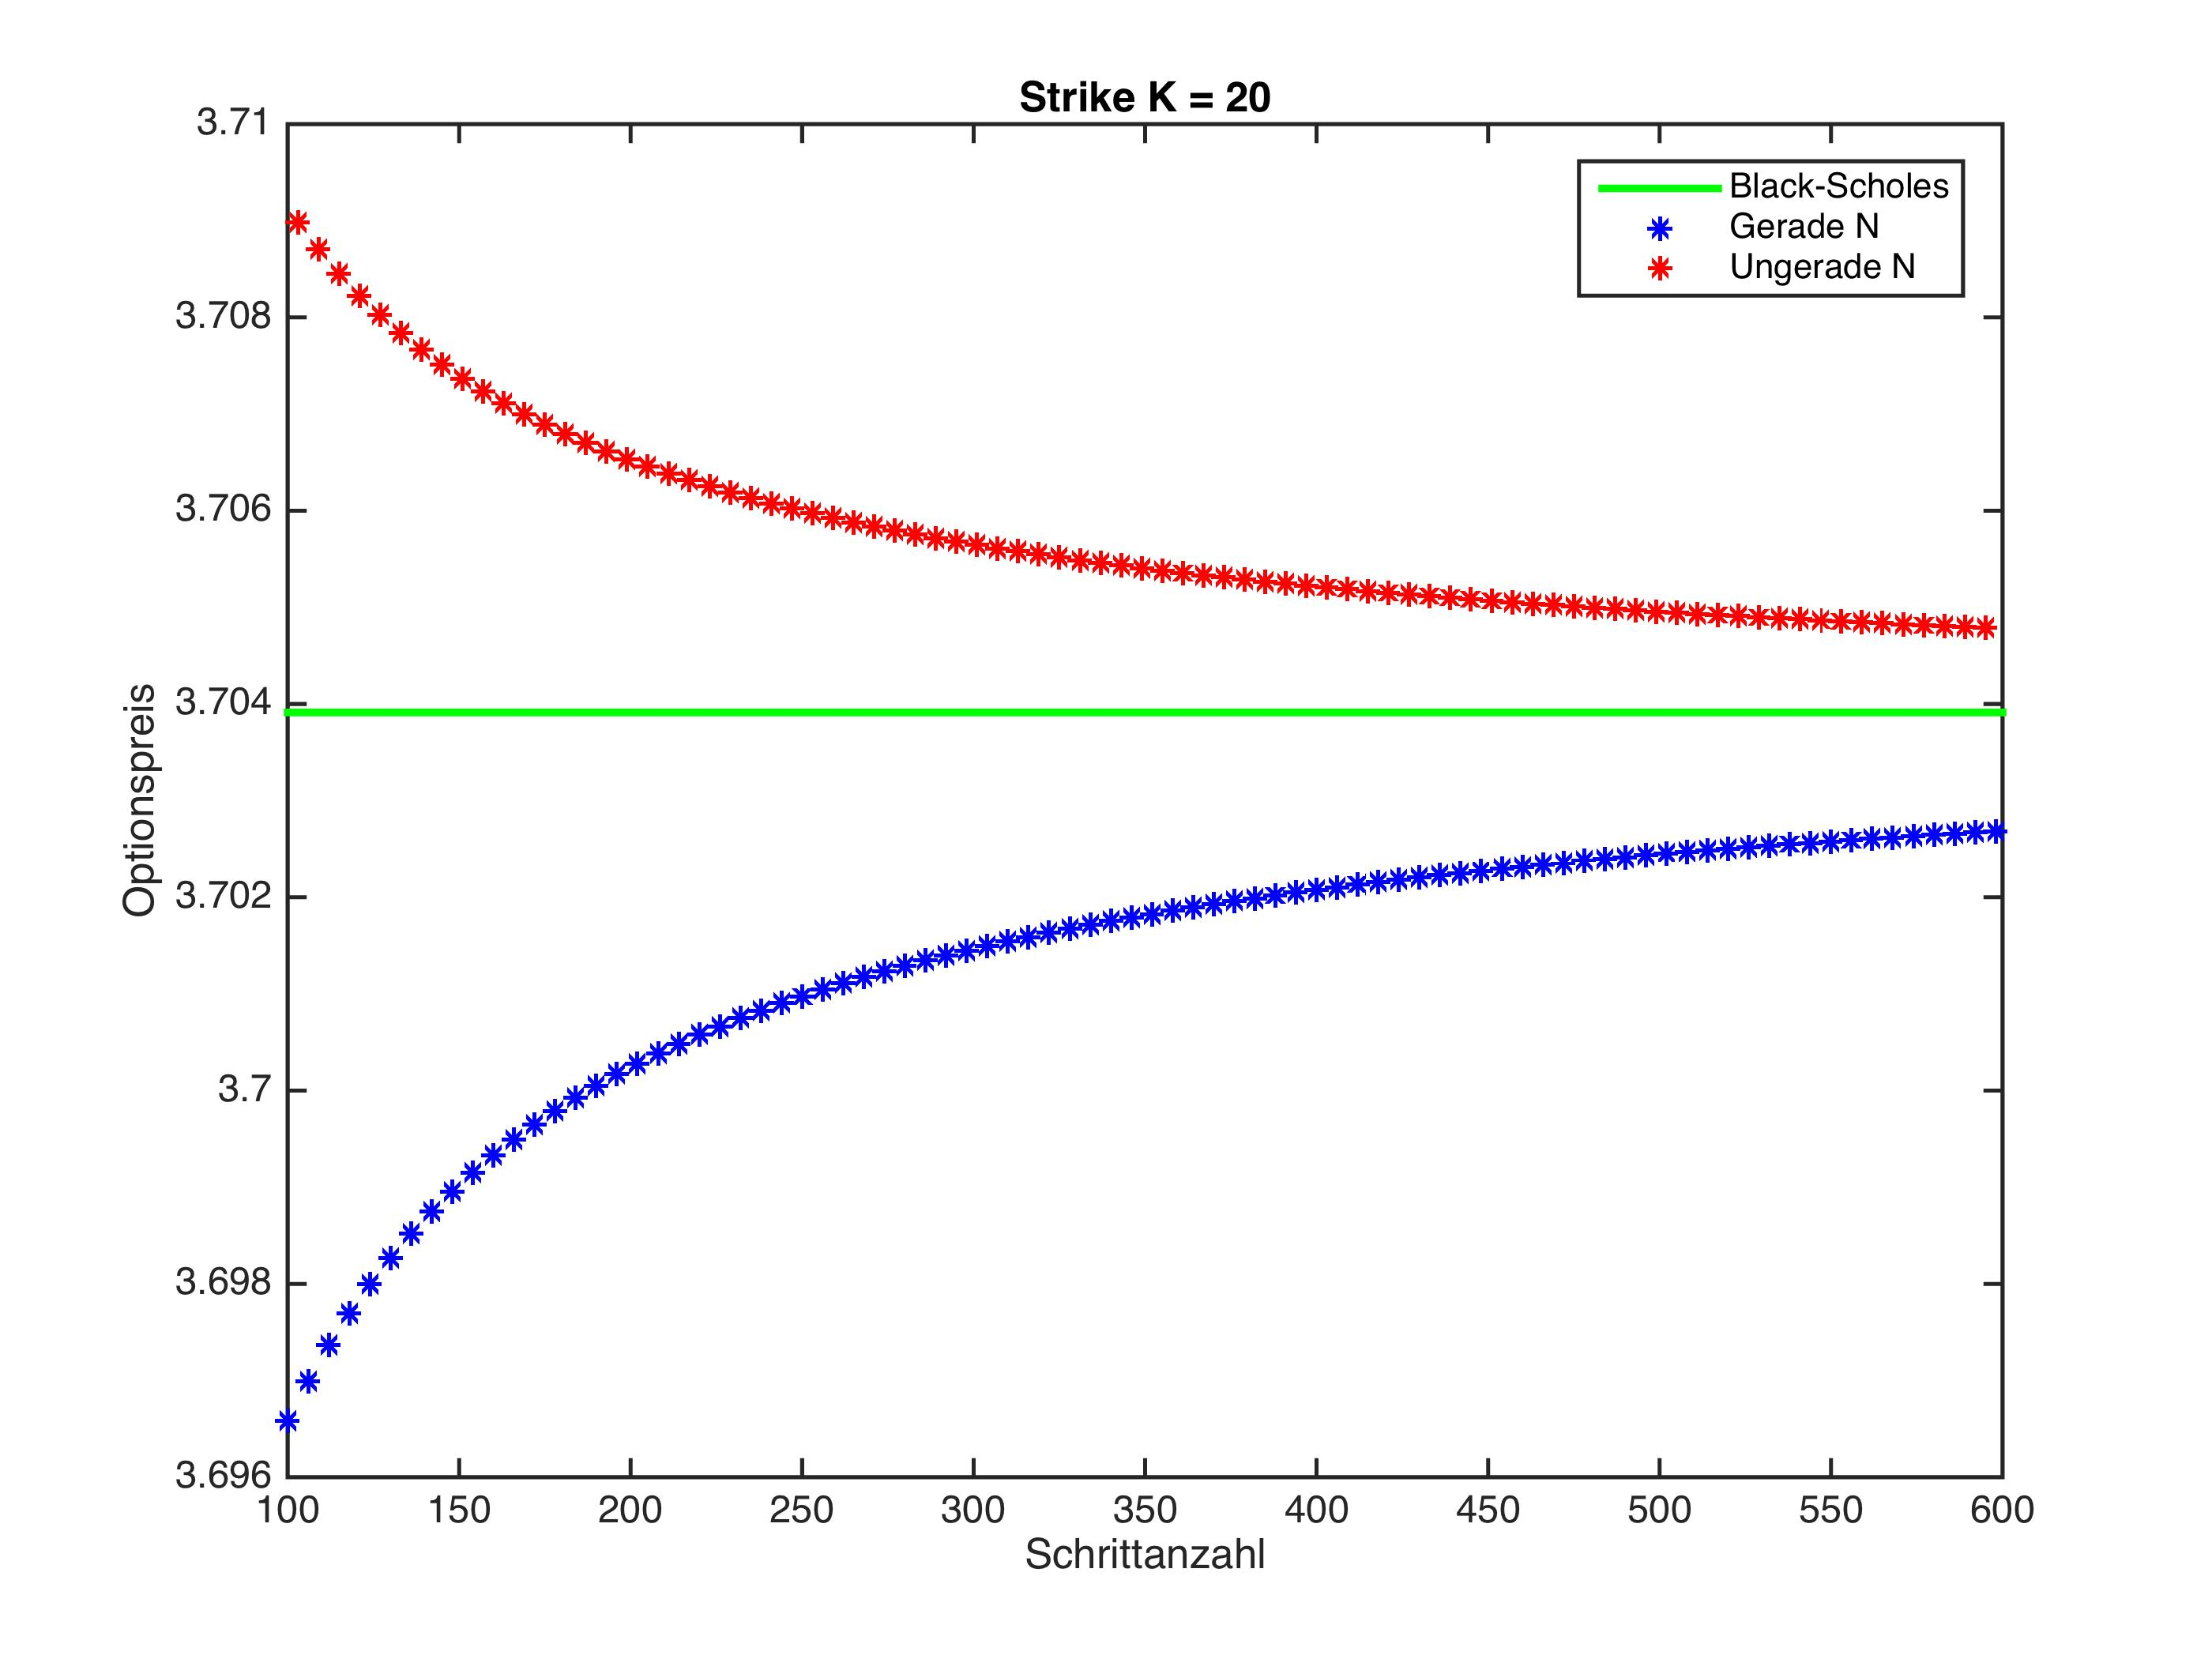
\includegraphics[width=0.45\textwidth]{KonvergenzCall20.jpg}
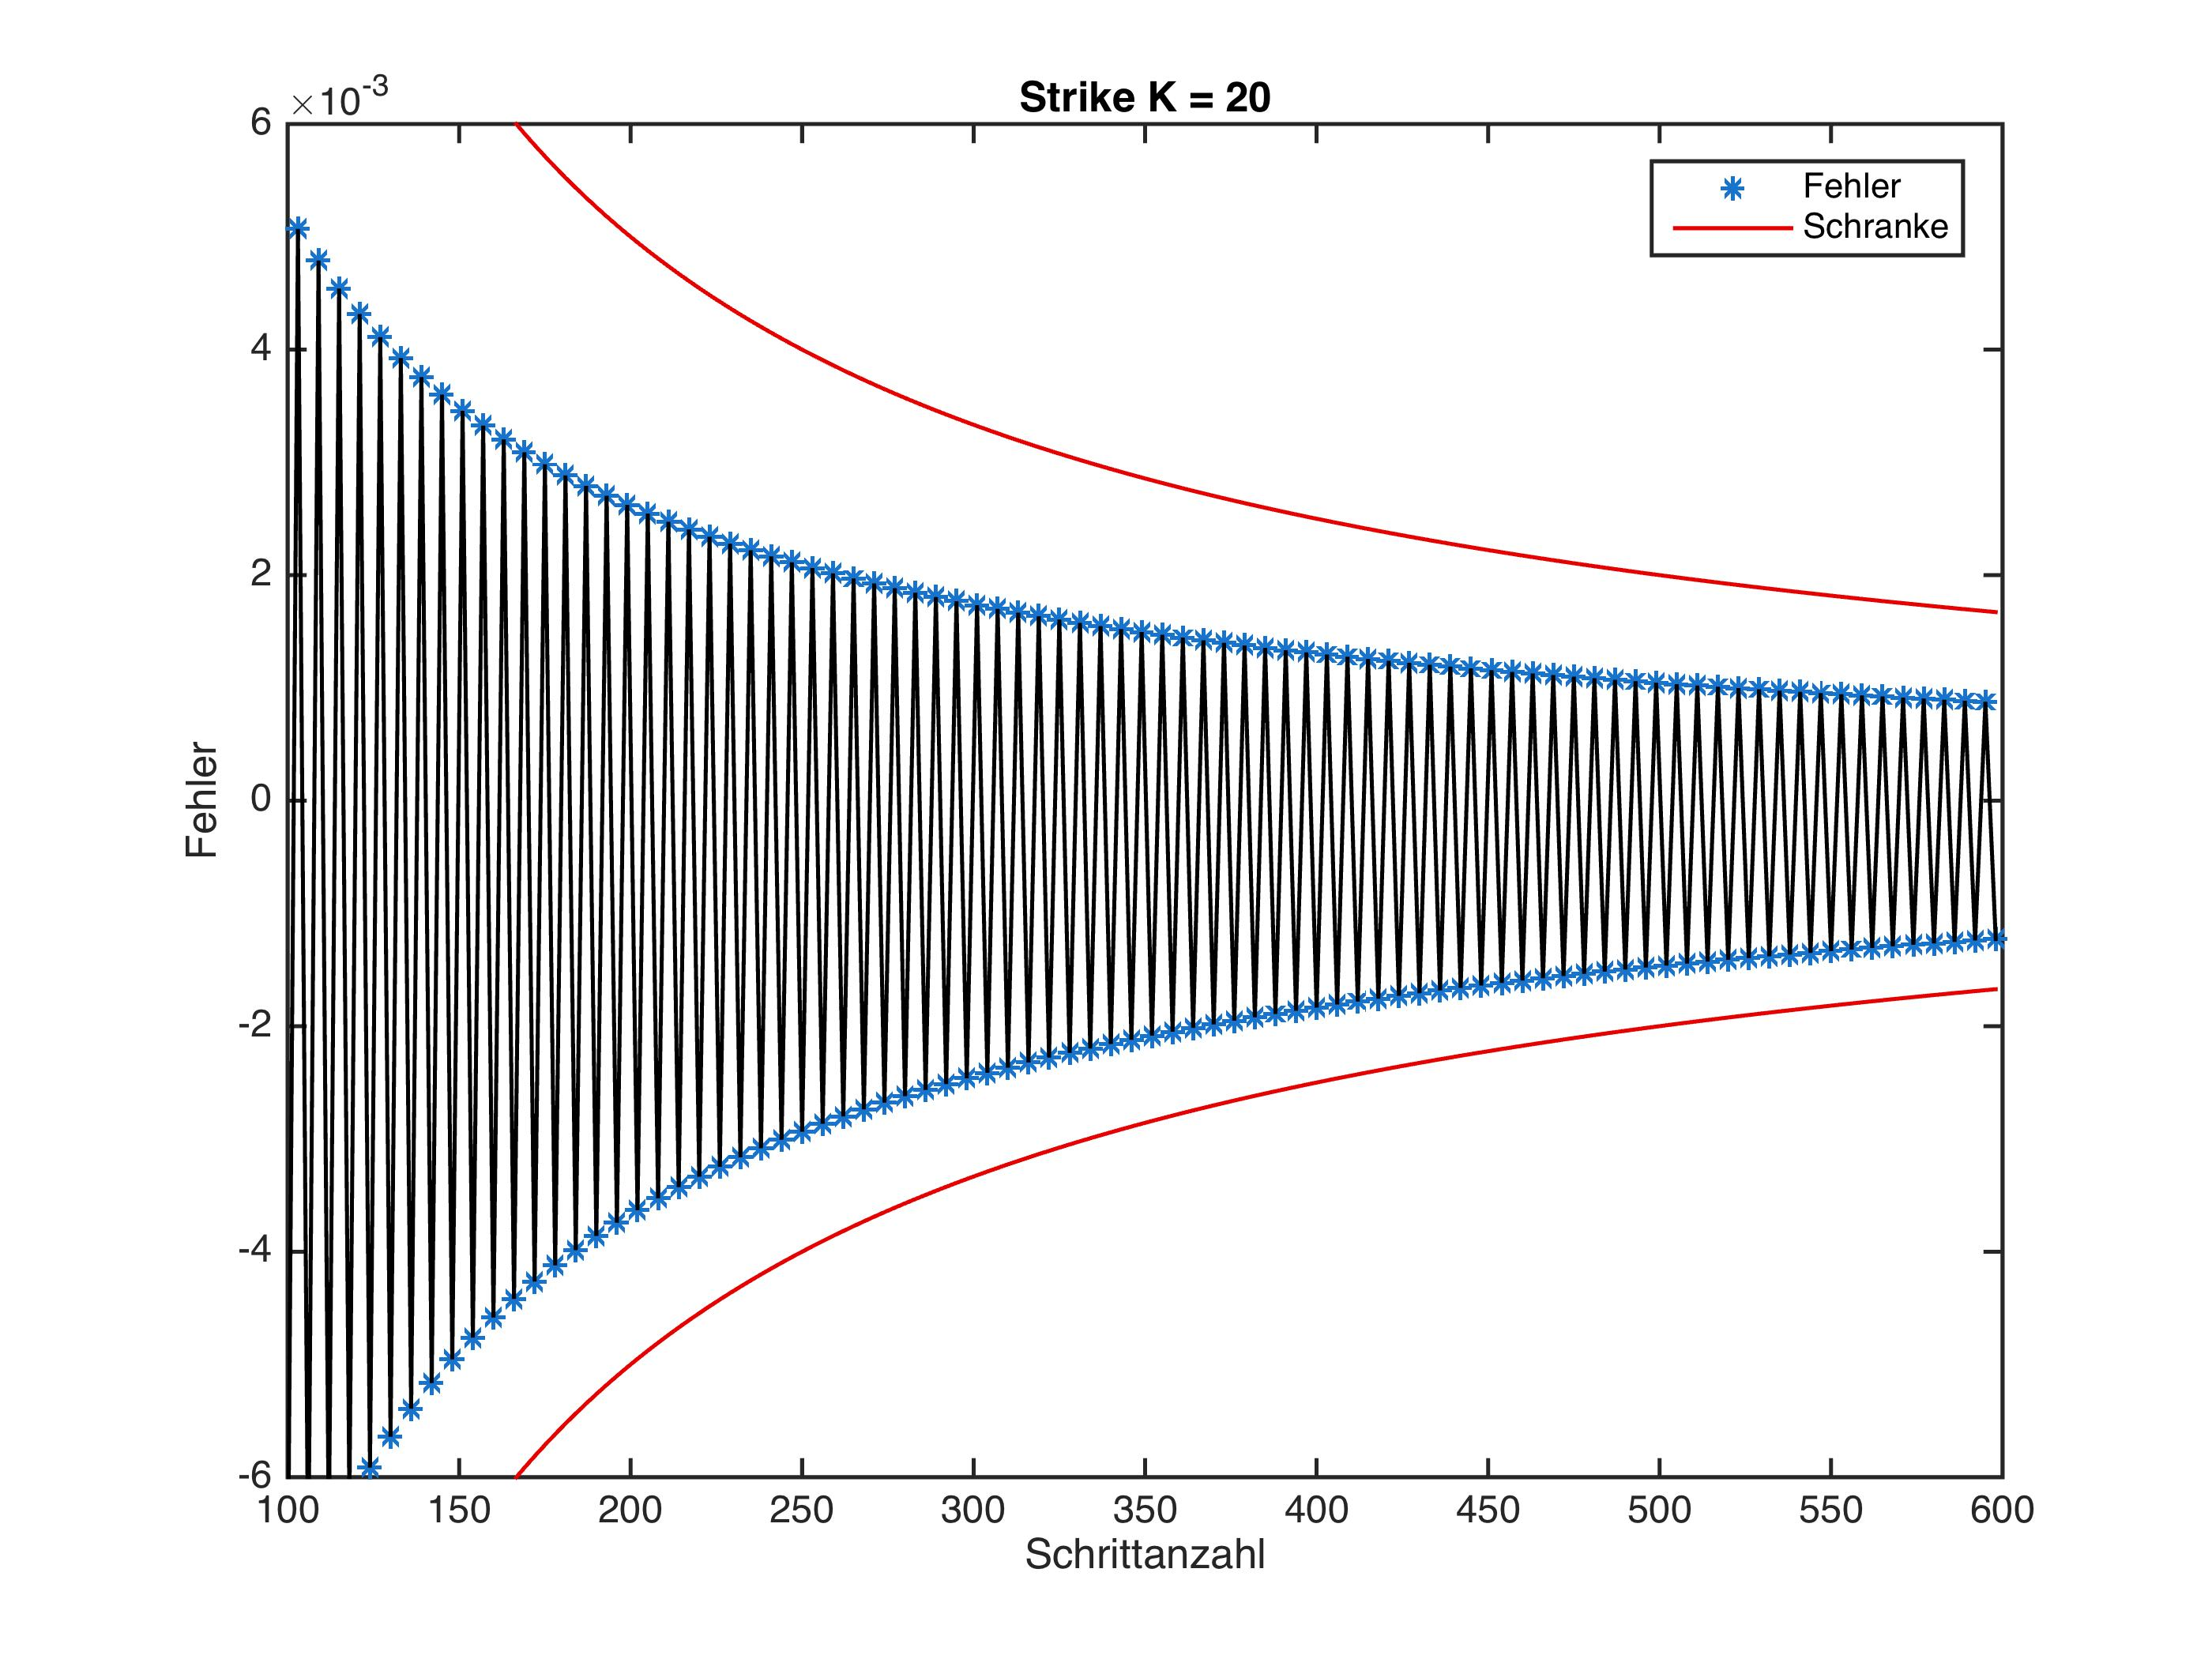
\includegraphics[width=0.45\textwidth]{FehlerCall20.jpg}
\caption{Konvergenz und Fehlerdarstellung für eine Europäische Call-Option mit $K=18$ bzw. $K=20$, $S_0=20$, $r = 0.1$, $\sigma = 0.35$ und $T=1$. Die Fehlerschranke ist $\frac{1}{N}$.}
\end{figure}\\
Was sofort auffällt, ist die unterschiedliche Konvergenz für die verschiedenen $K$. Während wir für $K=20$ eine jeweils monotone Konvergenz für gerade und ungerade Schrittanzahlen, sieht man für $K=18$ eine Art \glqq sprunghafte\grqq\, Konvergenz. Da $u_n$ und $d_n$ gegen $1$ konvergieren, konzentrieren sich immer mehr finale Knoten des Binomialbaums um $S_0$. 
\begin{figure}[h]
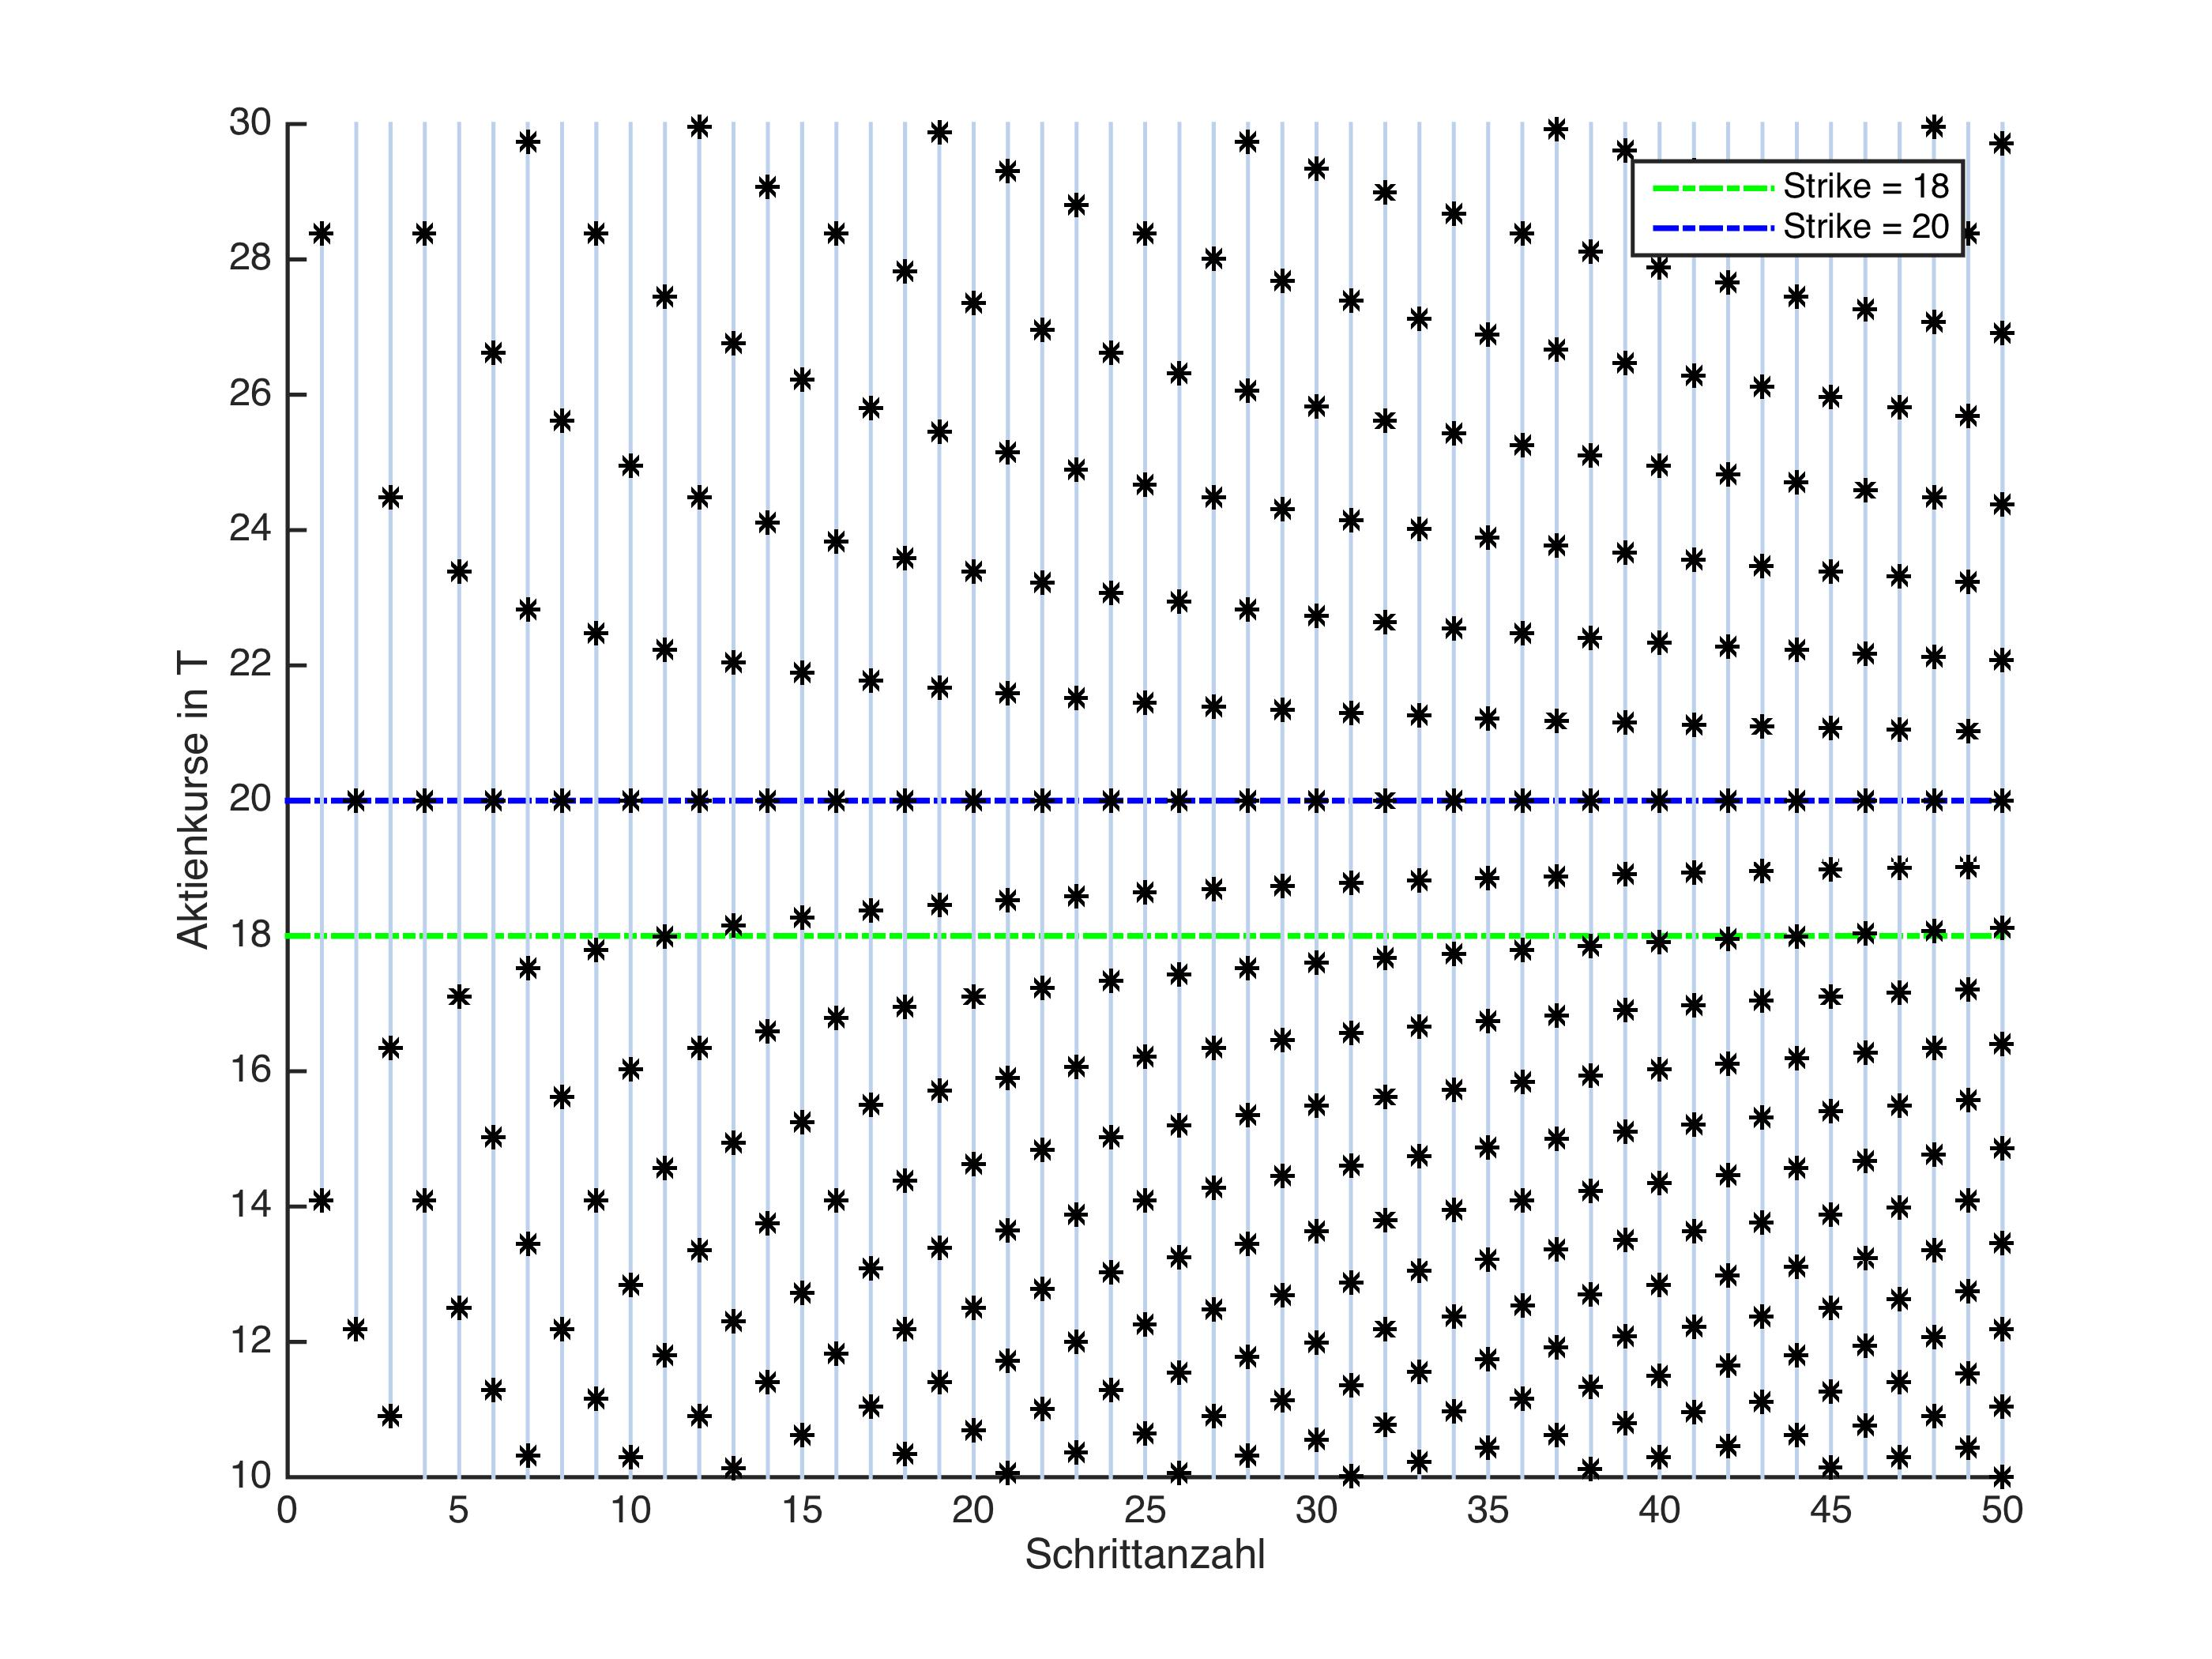
\includegraphics[width=0.9\textwidth]{Verjuengung.jpg}
\caption{Verjüngung der Endknoten in $T$ mit steigender Schrittanzahl.}
\end{figure}

Durch diese Verjüngung alterniert der Abstand des Strike Price $K=18$ zum nächsten Knoten im Endzeitpunkt $T$, wodurch die Sprünge in der Konvergenz erklärt werden \cite{LeisenReimer}. Je größer dabei der Abstand ist, desto mehr wird die Option überbewertet. Wenn $K=S_0$, so liegt wegen $u\cdot d = 1$ der Strike Price für gerade $N$ genau auf einem finalen Knoten und für ungerade $N$ genau zwischen zwei Knoten, was die jeweils monotone Konvergenz für $K=20$ erklärt.


%%%%%%%%% BLACK SCHOLES BEISPIELE %%%%%%%%%%%%%%%%%%%%%%%
\newpage
\section{Black-Scholes-Modell}
\label{BSP:BSModell}
Im Folgenden sind jeweils die Werte einer Put- und einer Call-Option im Vergleich zwischen Europäischer und Amerikanischer Version geplottet. 
\begin{figure}[h]
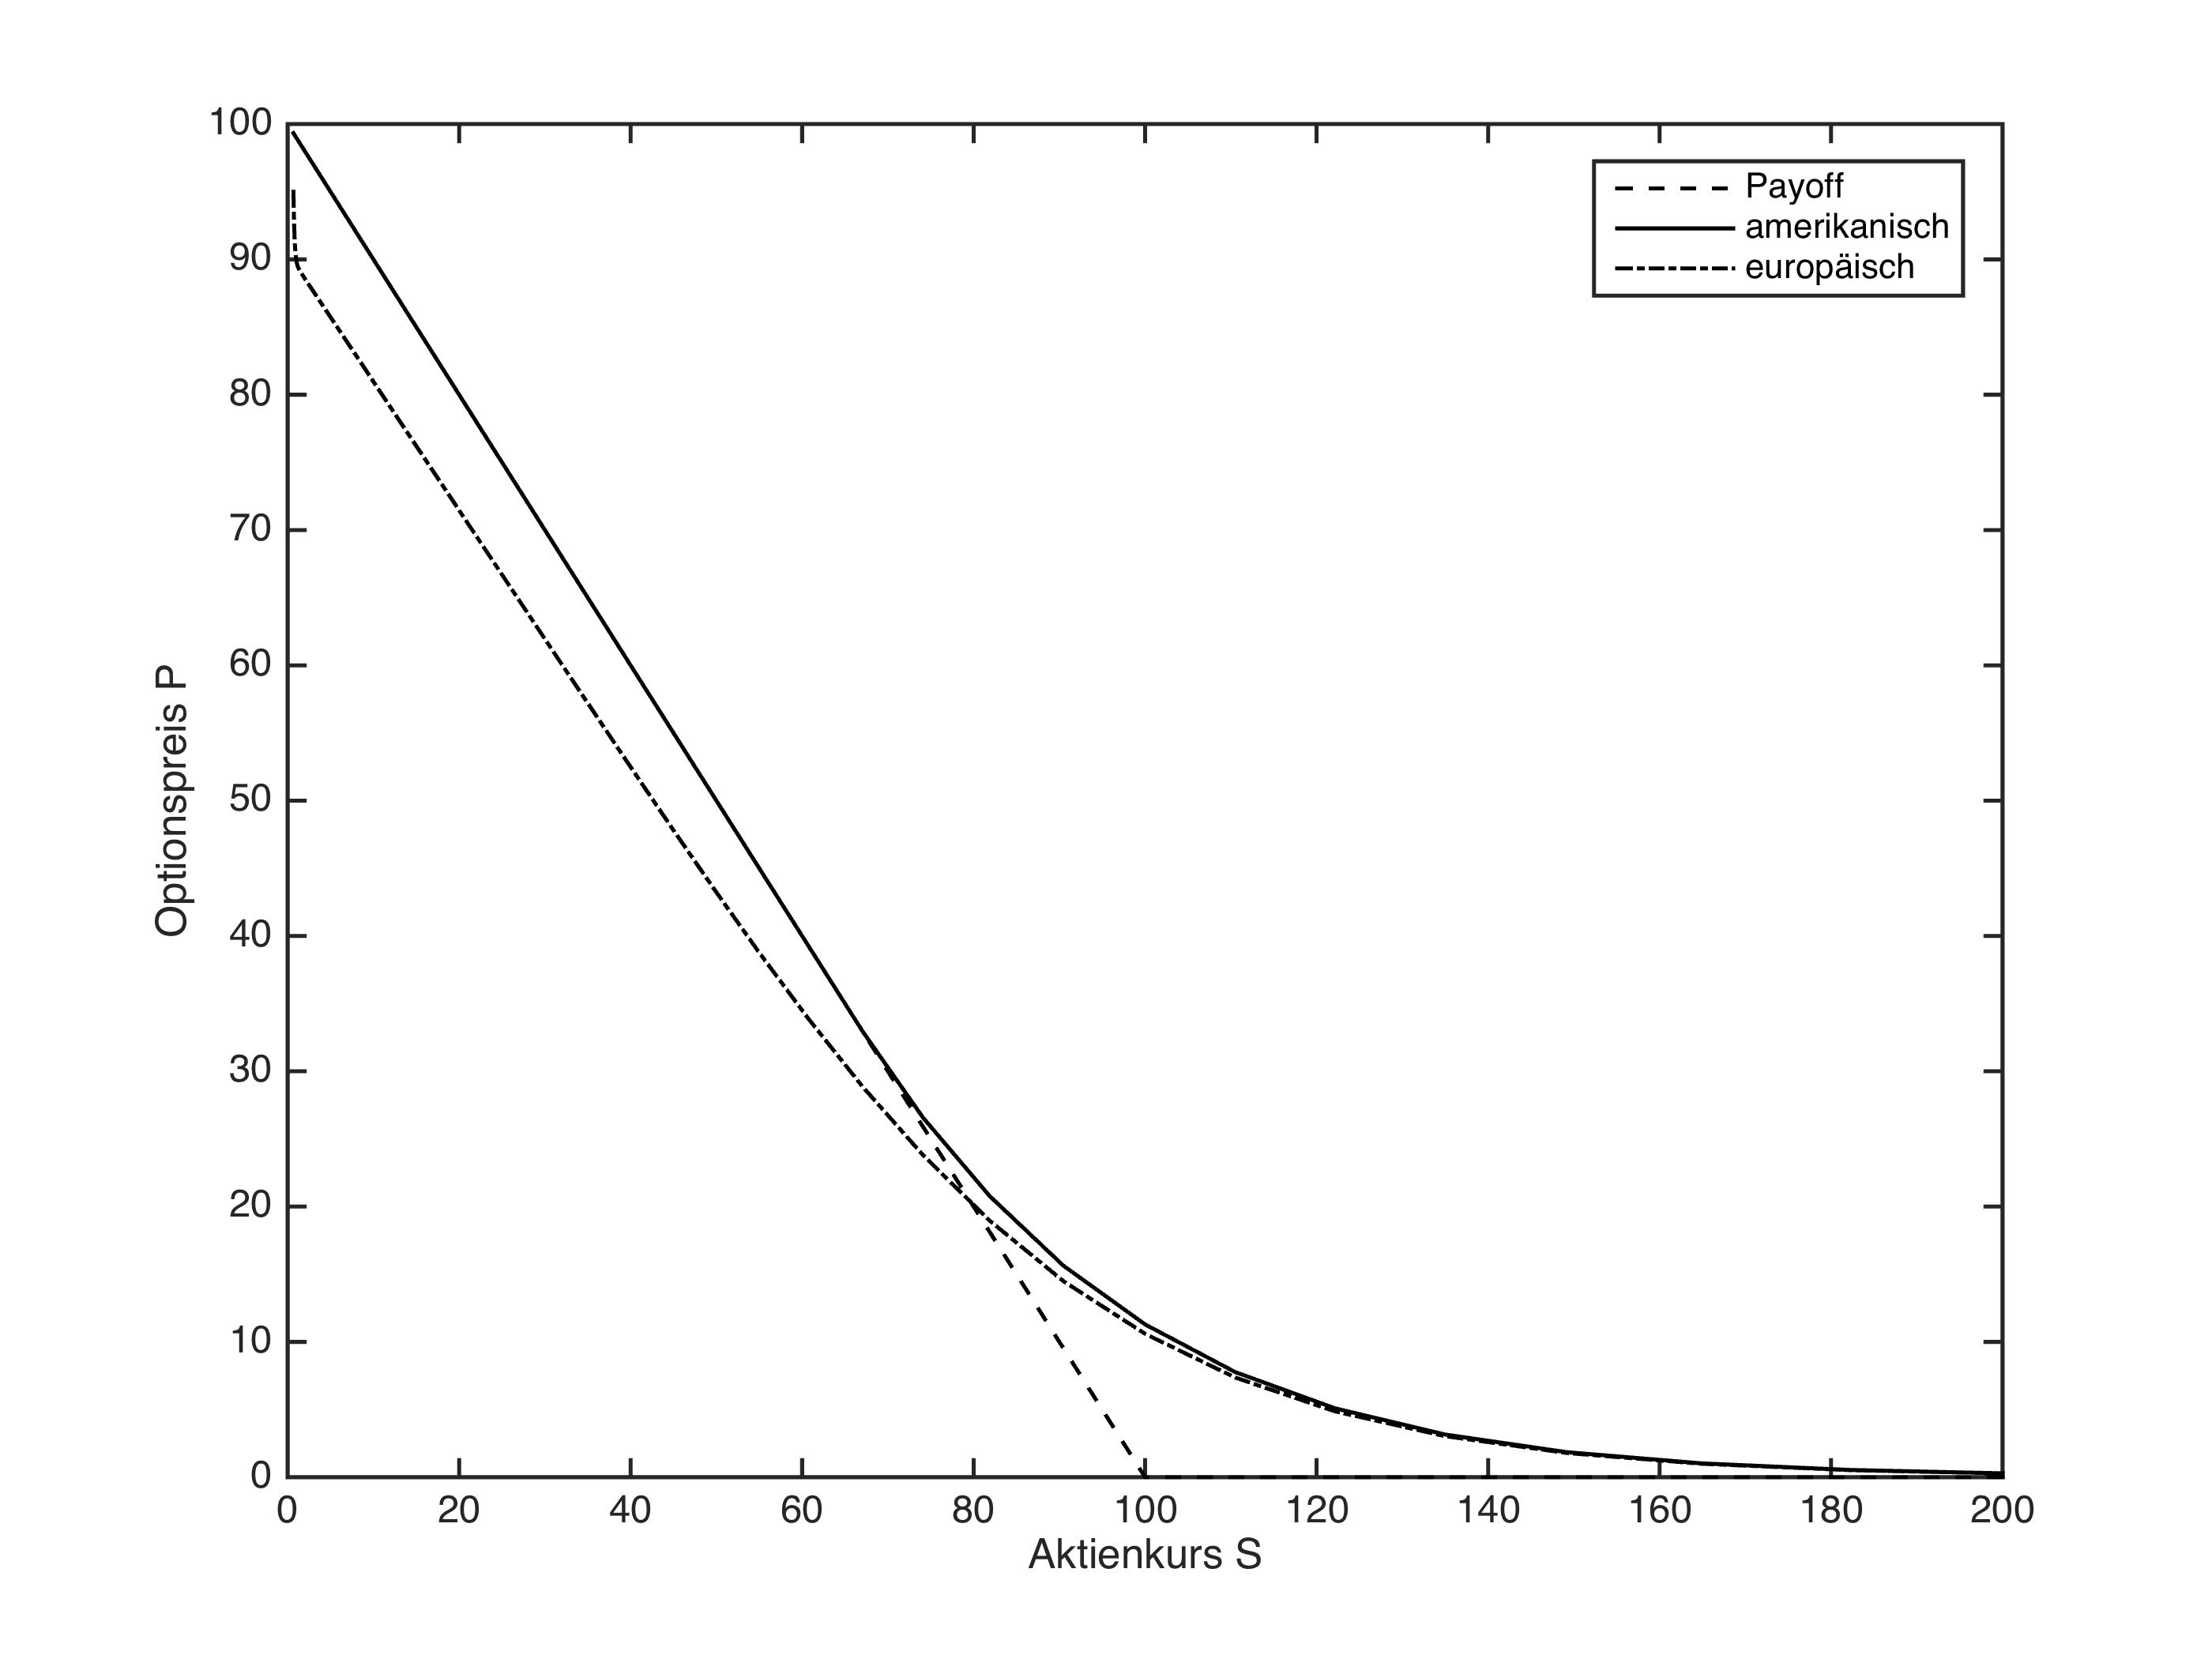
\includegraphics[width=0.9\textwidth]{PlotPutOption.jpg}
\caption{Wert einer Europäischen und einer Amerikanischen Put-Option mit $r = 0.1$, $\sigma^2 = 0.35$, $T=1$ und $D_0 = 0.05$. Berechnet durch Diskretisierung der Wärmeleitungsgleichung mit $a=5$, $M=5$ und $N=100$.}
\end{figure}
Man sieht direkt, dass der Wert der Amerikanischen Option immer größer ist als der der Europäischen. Es ist zu erkennen, dass sich die Optionswerte nicht nur in den Aktienkursen, zu denen eine Ausübung sinnvoll wäre, unterscheiden, sondern auch danach bzw. davor. Dies erscheint auch plausibel, da es für einen Aktienkurs nahe der Ausübungsgrenze wahrscheinlich ist, dass vom frühzeitigen Ausübungsrecht der Amerikanischen Option gebraucht gemacht wird. Diese Grenze, den im Komplementaritätsproblem (\ref{BS:LKP1})-(\ref{BS:LKP3}) implizit formulierten freien Randwert $S_f(t)$, kann man im Schaubild der Optionswerte nur schwer ablesen, allderdings lässt er sich innerhalb der Matlab Funktion durch Vergleich der Lösung $V(S_0,0)$ mit $\Lambda(S_0)$ mit geringem Aufwand ausgeben. Es gilt $S_f^p(0)\approx 74.0818$ für die Put-Option und $S_f^c(0) \approx 201.3753$. Die Approximation von $S_f^c$ ist allerdings kritisch zu betrachten, da die Gitterpunkte durch die gewählte Approximation für $S>K$ einen sehr großen Abstand haben. 
\begin{figure}[h]
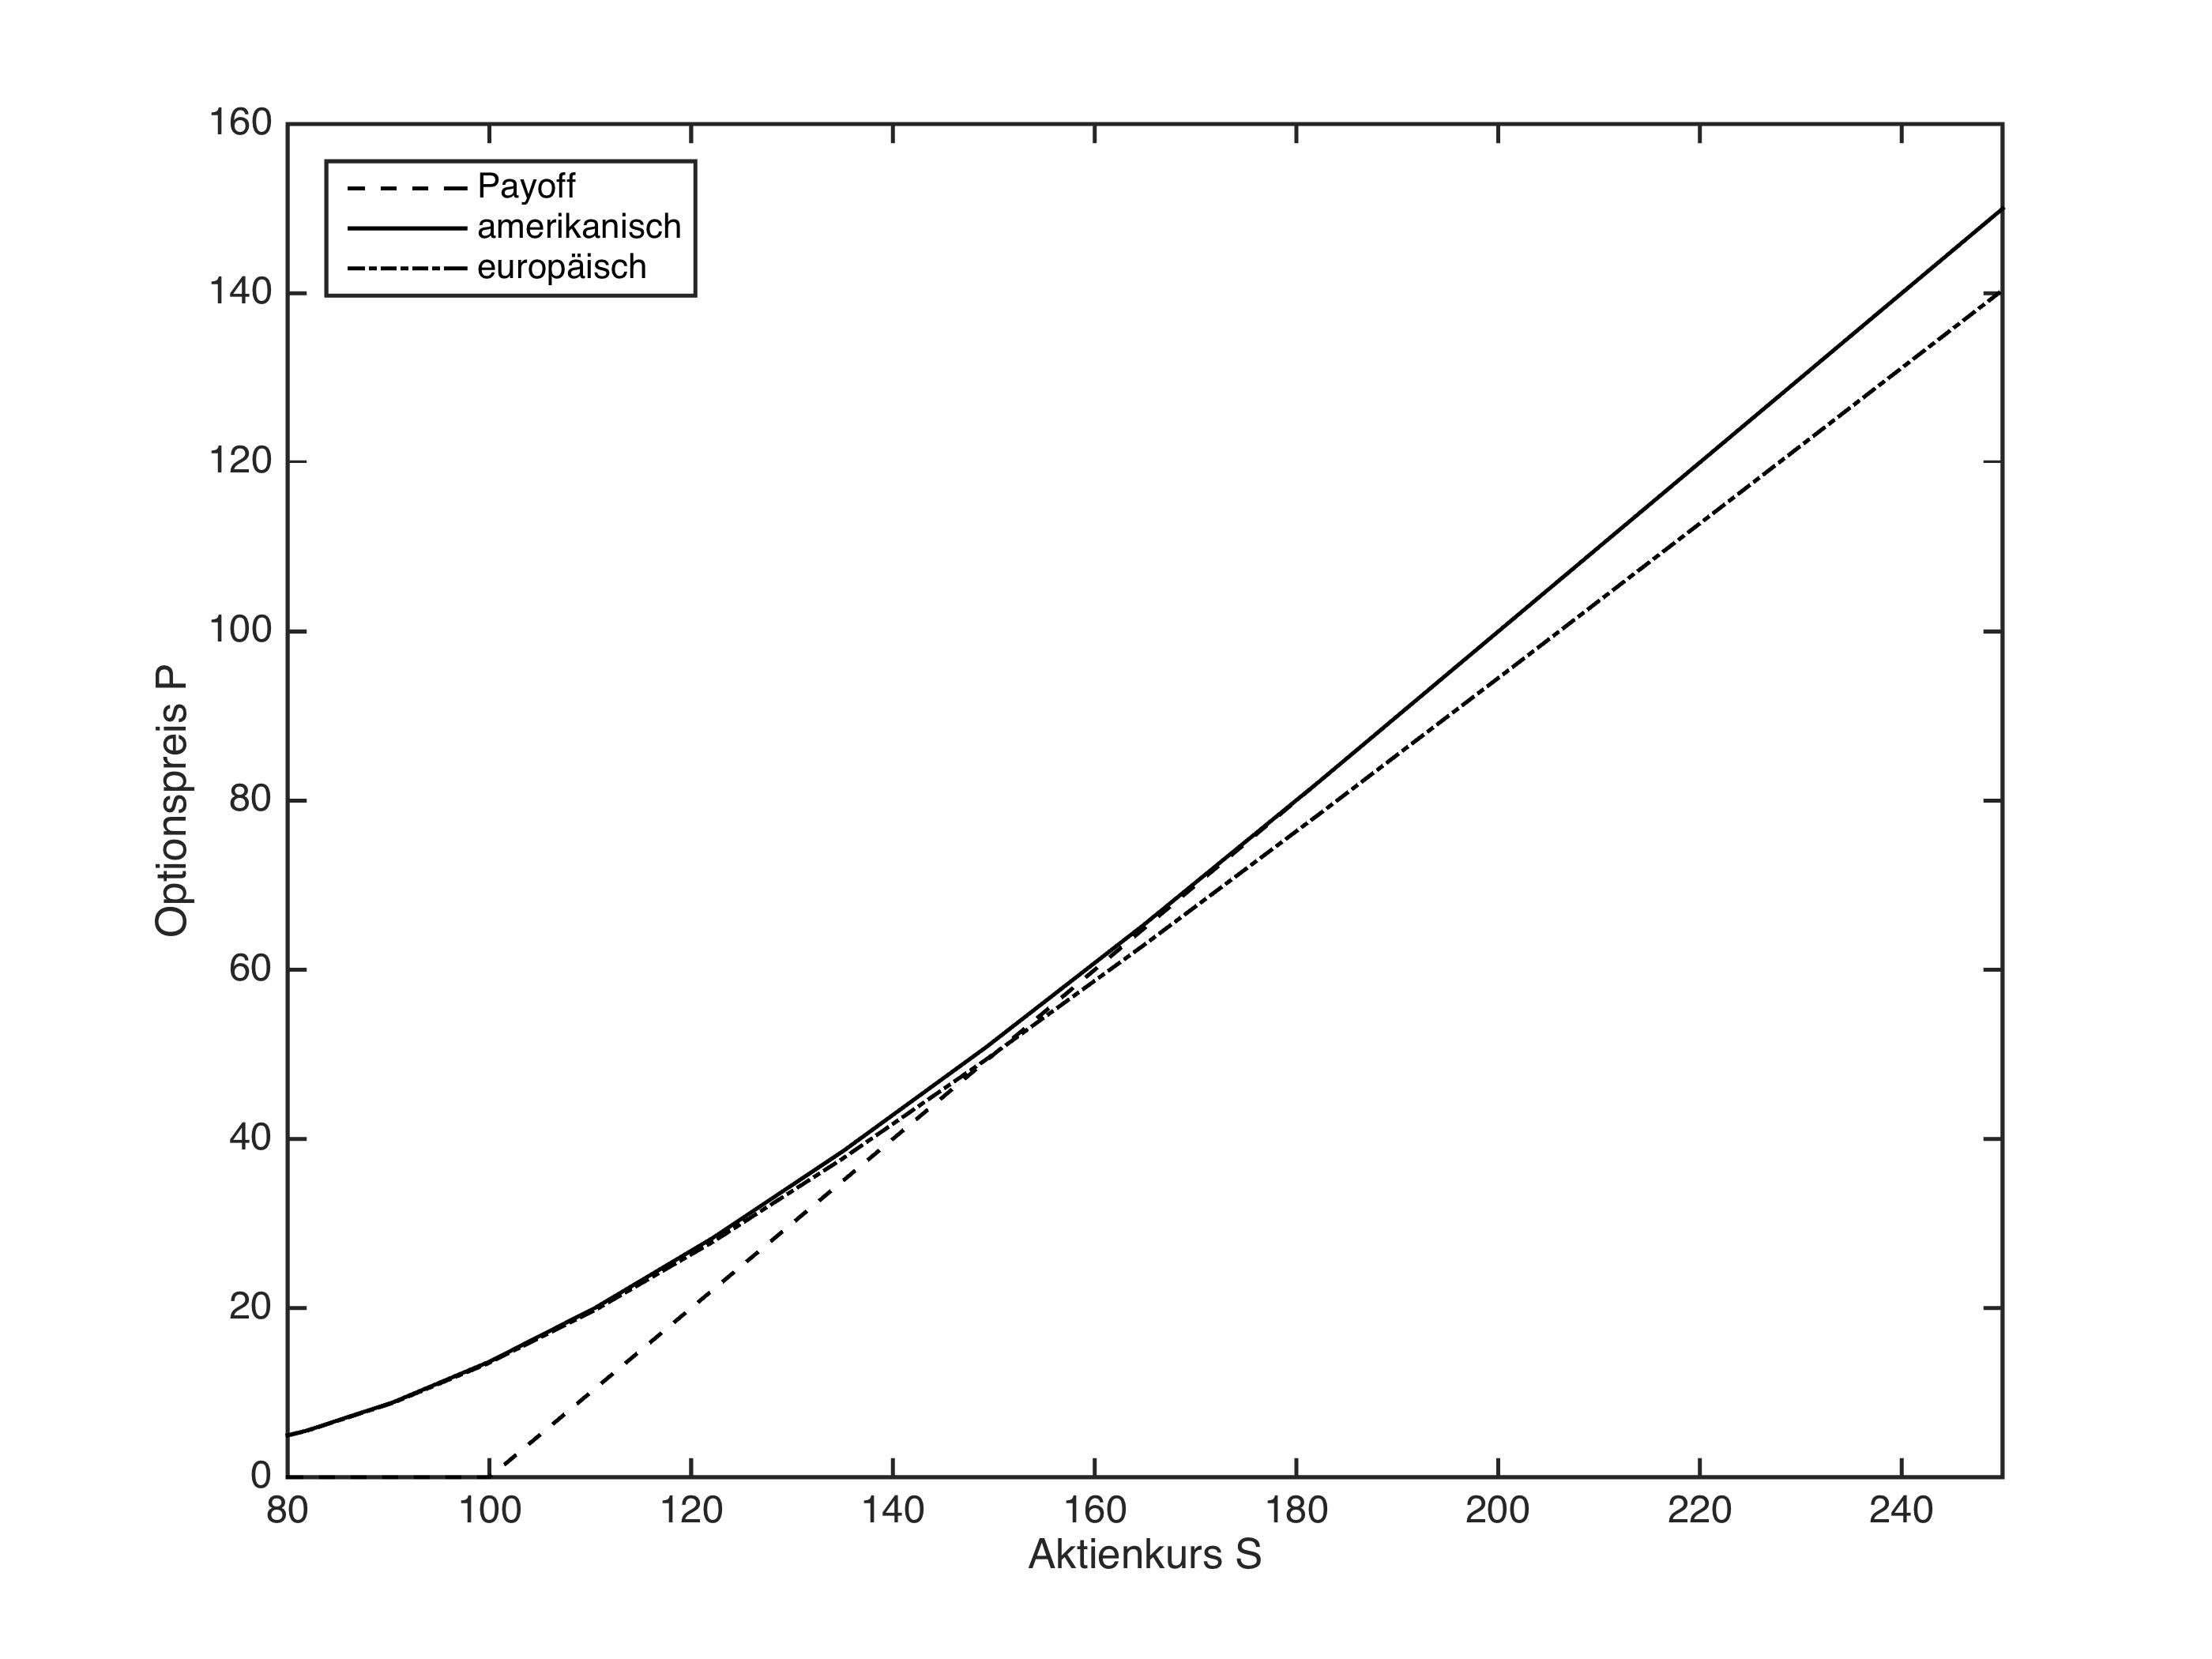
\includegraphics[width=0.9\textwidth]{PlotCallOption.jpg}
\caption{Wert einer Europäischen und einer Amerikanischen Call-Option mit $r = 0.1$, $\sigma^2 = 0.35$, $T=1$ und $D_0 = 0.08$. Berechnet durch Diskretisierung der Wärmeleitungsgleichung mit $a=5$, $M=5$ und $N=100$.}
\end{figure}
Möglichkeiten, die Approximation zu verbessern wären zum Einen eine Erhöhung der Schrittanzahl (was aber den Rechenaufwand und damit die Laufzeit stark erhöht), zum Anderen mithilfe eines aus dem Plot abgelesenen approximativen $S_f^c$ eine verbesserte Wahl des Gitters. Man kann dann zu gleicher Anzahl an Gitterpunkten die Diskretisierung z.B. nur auf $\left[-a,k\cdot a\right]$ (für geeignetes $k\in \left(0,1\right]$) durchführen und erhält damit eine feinere Darstellung für $K\leq S \leq S_f^c$. Mit $k=0.2$ erhalten wir $S_f^c \approx 185.8928$, was eine bessere Approximation an den \glqq wahren\grqq \, Randwert $\tilde S_f^c = 181.7387$ (berechnet mit $N=10\,000$ Gitterpunkten auf $\left[-a,0.2\cdot a\right]$) liefert.

%In der folgenden Abbildung lassen sich sowohl der in $t$ fallende freie Randwert $S_f(t)$, also auch die
%\begin{figure}[h]
%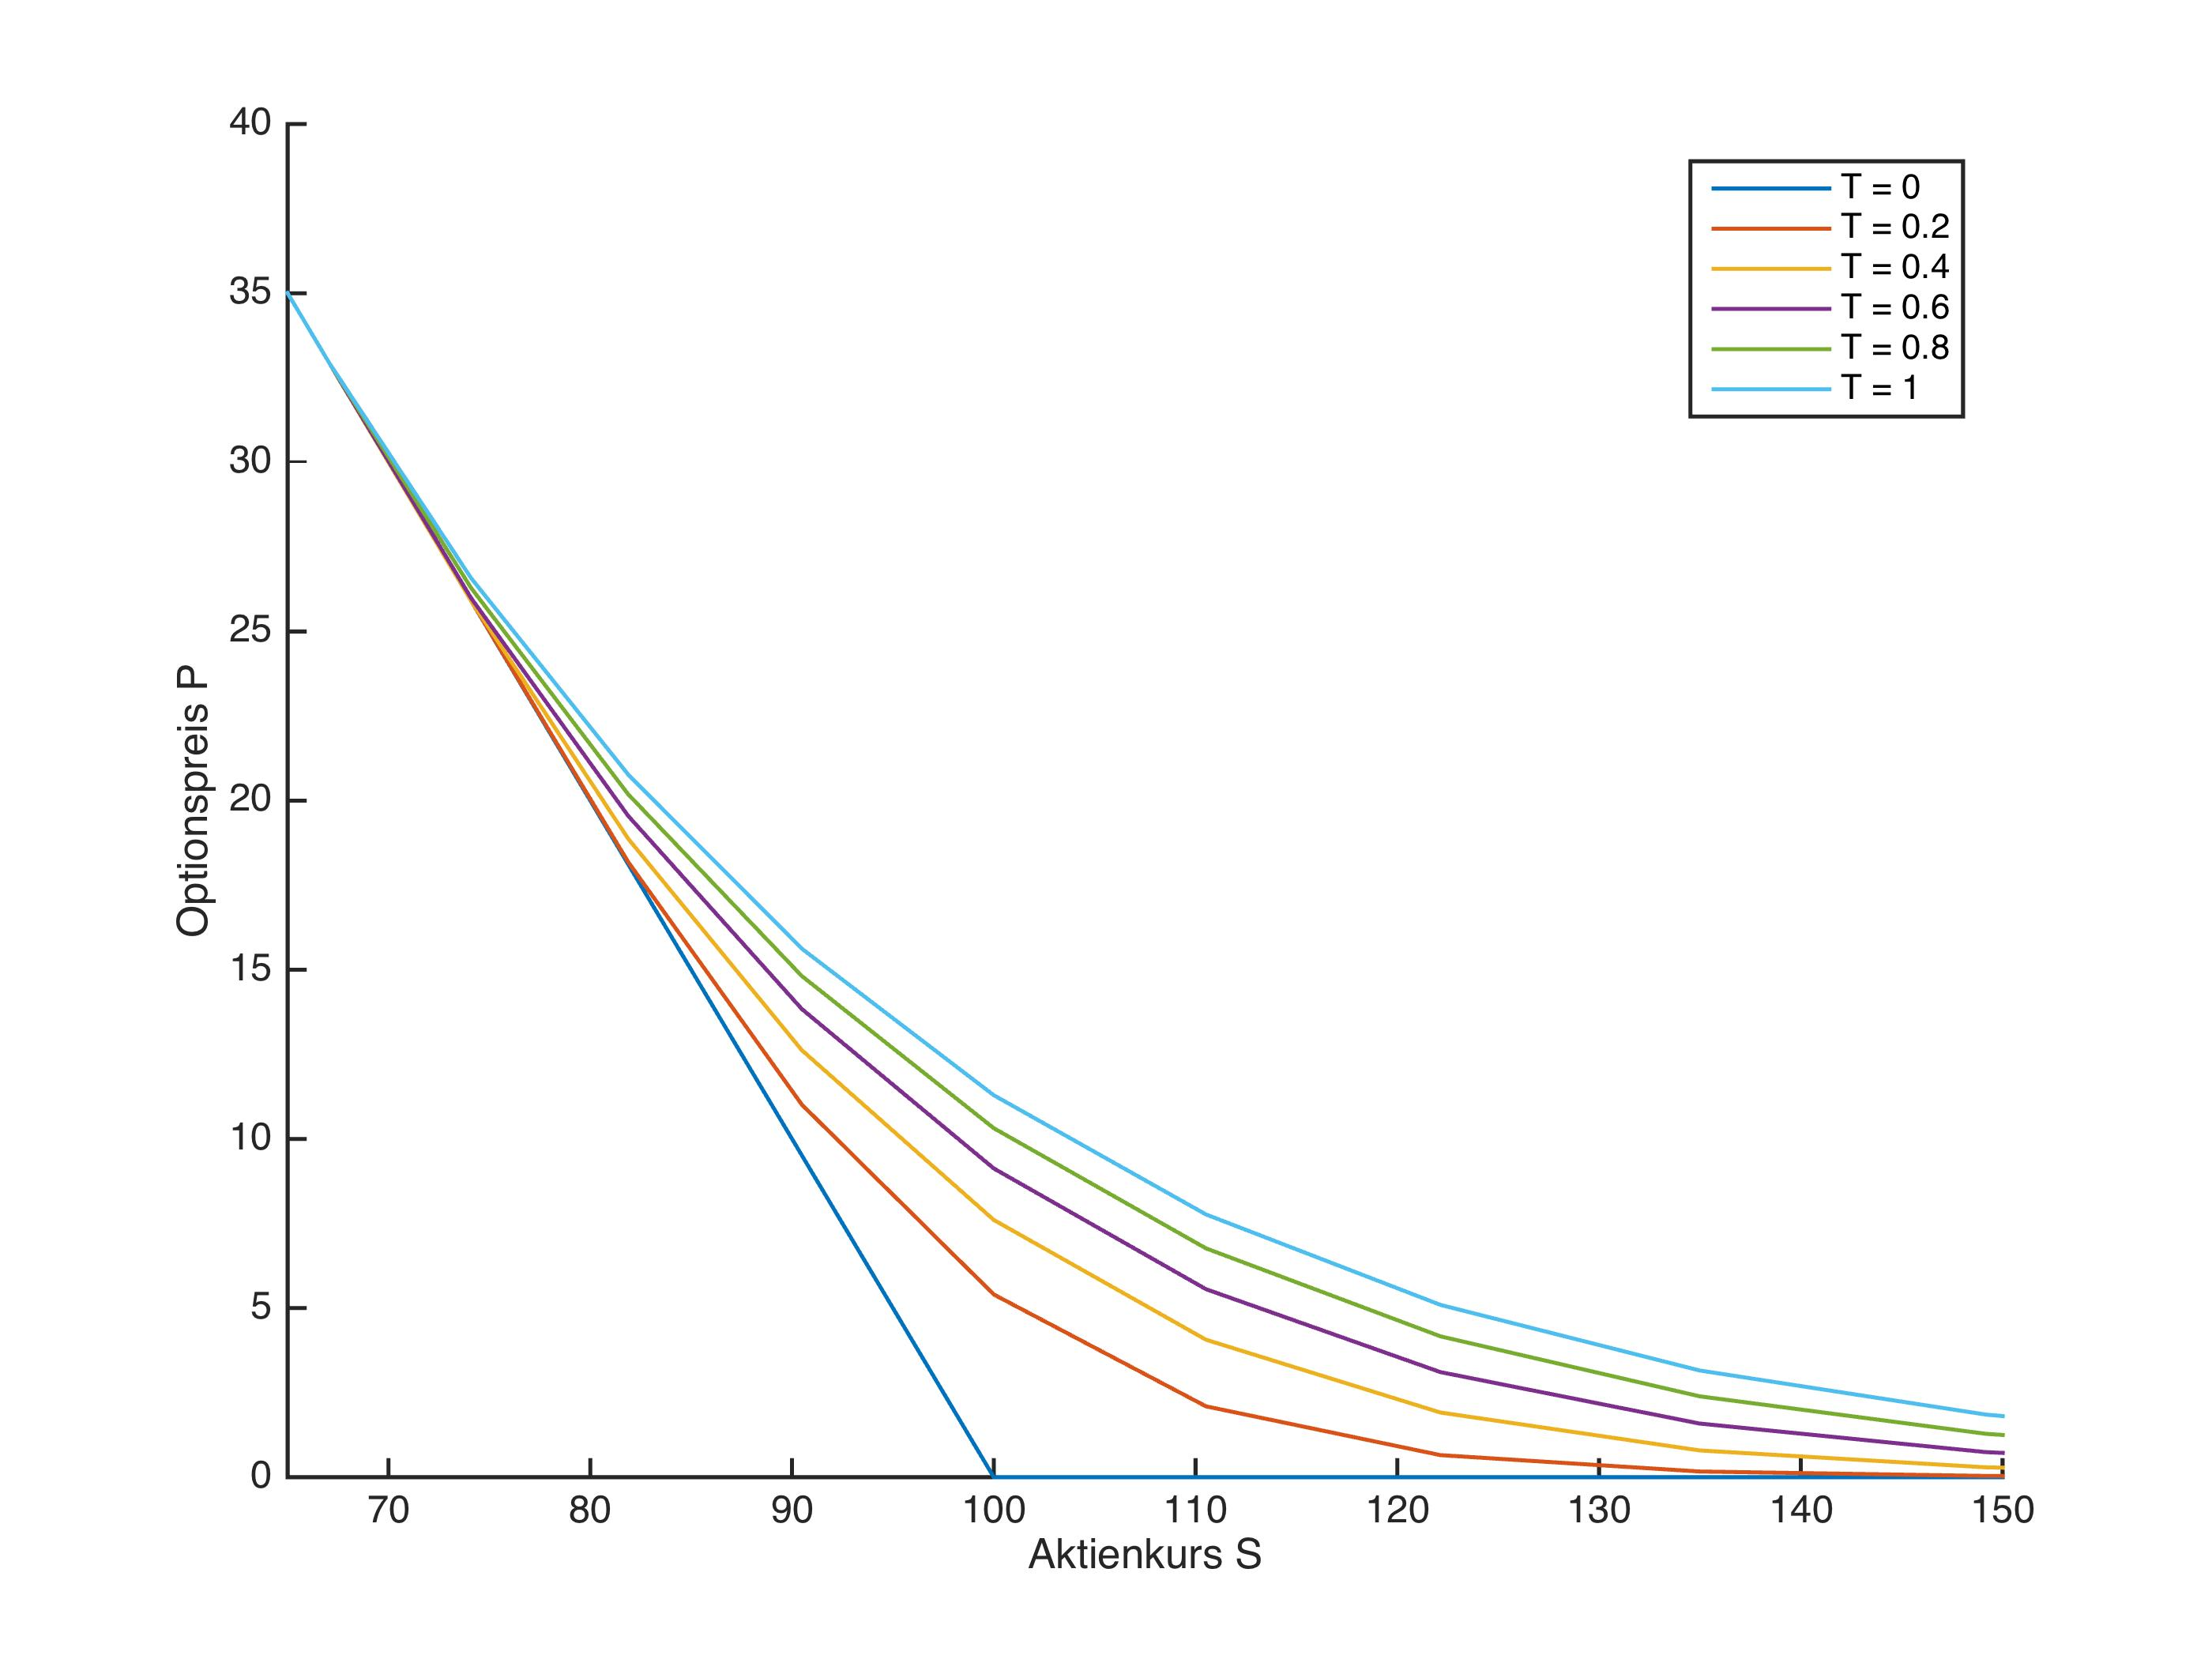
\includegraphics[width=0.9\textwidth]{AmerikanischeZeitverlauf.jpg}
%\caption{Zeitlicher Verlauf einer Amerikanischen Put-Option mit $r = 0.1$, $\sigma^2 = 0.35$, $T=1$ und $D_0 = 0.08$. Berechnet durch Diskretisierung der Wärmeleitungsgleichung mit $a=5$, $M=5$ und $N=100$.}
%\end{figure}

